\documentclass[tikz, border=4pt]{standalone}
\usepackage{tikz}
\usetikzlibrary{angles, quotes}
\begin{document}
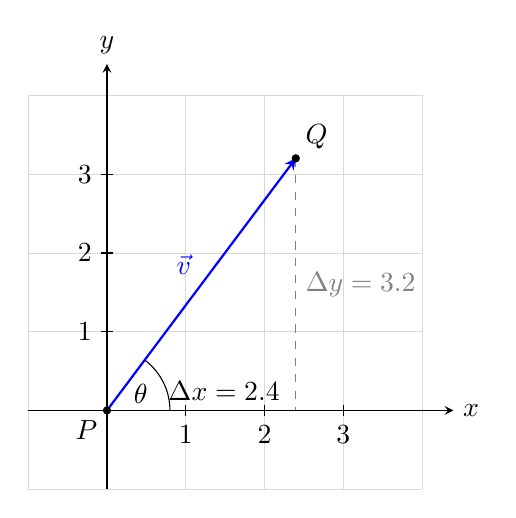
\begin{tikzpicture}[x=1cm, y=1cm]
  \begin{scope}[shift={(1.05,-4.95)}]
    % the vector v = (\vlen; \vang°): drag Q, or change the values
    \pgfmathsetmacro{\vlen}{4}
    \pgfmathsetmacro{\vang}{53.17}
    \pgfmathsetmacro{\dx}{\vlen*cos(\vang)}
    \pgfmathsetmacro{\dy}{\vlen*sin(\vang)}
    \draw[step=1, very thin, black!15] (-1,-1) grid (4,4);
    \draw[-stealth] (-1,0) -- (4.4,0) node[right]{$x$};
    \draw[-stealth] (0,-1) -- (0,4.4) node[above]{$y$};
    \foreach \x in {1,...,3} \draw (\x,2pt) -- (\x,-2pt) node[below]{$\x$};
    \foreach \y in {1,...,3} \draw (2pt,\y) -- (-2pt,\y) node[left]{$\y$};
    \coordinate (P) at (0,0);
    \coordinate (Q) at (\vang:\vlen);
    \coordinate (R) at (Q |- P);
    \draw[dashed, gray] (Q) -- (R) node[midway, right]{$\Delta y = \pgfmathprintnumber[fixed,precision=2]{\dy}$};
    \path (P) -- (R) node[pos=0.62, above]{$\Delta x = \pgfmathprintnumber[fixed,precision=2]{\dx}$};
    \pic[draw, "$\theta$", angle radius=8mm] {angle = R--P--Q};
    \draw[-stealth, thick, blue] (P) -- (Q) node[midway, above left]{$\vec{v}$};
    \fill (P) circle (1.5pt) node[below left]{$P$};
    \fill (Q) circle (1.5pt) node[above right]{$Q$};
  \end{scope}
\end{tikzpicture}
\end{document}
